\documentclass[10pt,twocolumn]{article}

\usepackage[letterpaper,margin=0.75in]{geometry}
\usepackage{times}
\usepackage{graphicx}
\usepackage{booktabs}
\usepackage{multirow}
\usepackage{amsmath,amssymb}
\usepackage{amsthm}
\newtheorem{proposition}{Proposition}
\usepackage{caption}
\usepackage{microtype}
\usepackage[hidelinks]{hyperref}
\usepackage{xcolor}

\captionsetup{font=small,labelfont=bf}
\setlength{\parskip}{2pt}
\newcommand{\pp}{\,pp}

\title{\textbf{The Prior Is Not the Bottleneck:\\ Where Success Comes From in Guided Diffusion Motion Planning}}
\author{Anonymous\\ \small Workshop submission}
\date{}

\begin{document}
\twocolumn[
\begin{@twocolumnfalse}
\maketitle
\begin{abstract}
Guided diffusion is a popular paradigm for robot motion planning, and a steady
stream of work improves the \emph{generative prior}: better noise schedules,
richer trajectory representations, and environment conditioning. We present a
controlled study on Guided Polynomial Diffusion (GPD), re-implemented in the EDMP
codebase, showing that for a guided planner \textbf{the prior is largely not the
bottleneck}. Across five independent prior-side interventions---recalibrating the
noise schedule, increasing polynomial capacity, adding a smoothness penalty,
conditioning the denoiser on the scene with classifier-free guidance, and
training $5\times$ longer (to 1M steps)---planning success rate (SR) never
improves, with deltas ranging from statistically zero to small significant
\emph{decreases}, even when the interventions lower training loss or
reconstruction error. A failure-mode analysis isolates \emph{continuous (swept)}
infeasibility as the dominant residual failure. Acting on it, two interventions
on the \emph{feasibility machinery}---faithful-collision RRT stitching ($+17.4\pp$,
CI~{$[15.2,19.6]$}) and a trajectory-optimization repair ($+8.9\pp$, 95\% CI {$[7.6,10.2]$})---break the
plateau that no prior-side change could. A naive-seed control sharpens the claim:
the prior is \emph{necessary} as an initializer (a straight-line seed with the
same repair reaches only 55\% vs.\ 82\%) but \emph{improving} it does not help. The
repair lever transfers to a second planner (EDMP, $+7.6\pp$, CI~{$[5.2,9.9]$}) and collapses the
diagnosed swept-collision failure ($15.5\%\!\to\!3.0\%$). We argue the community's
effort is mis-allocated and release an open, GPU-native re-implementation with all
ablations.
\end{abstract}
\vspace{1.2em}
\end{@twocolumnfalse}
]

\begin{figure*}[t]
\centering
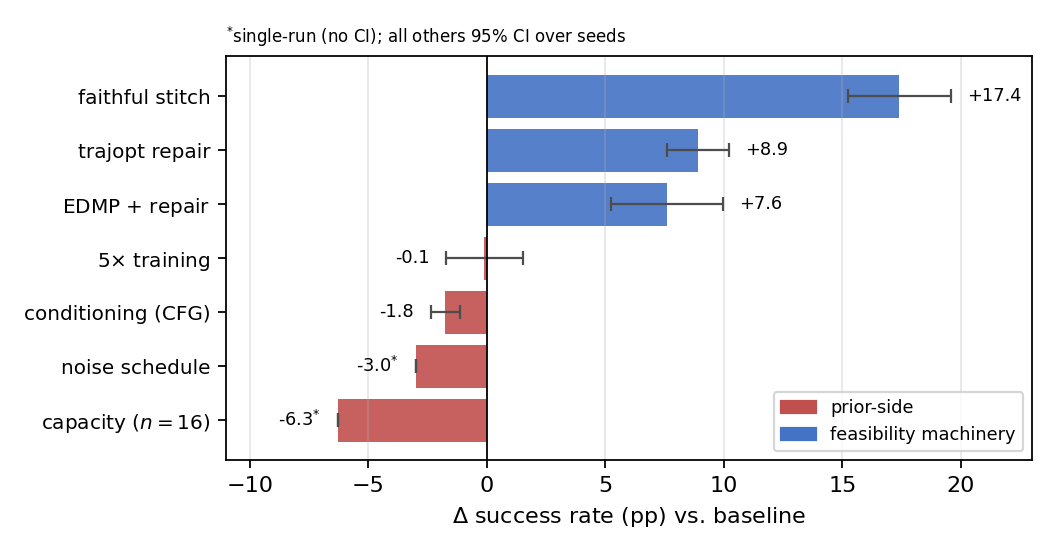
\includegraphics[width=0.66\textwidth]{figs/headline_deltas.png}
\caption{Success-rate change for each intervention on the hybrid benchmark. Every
prior-side change (red) is zero or negative; both feasibility-machinery levers
(blue) are large and positive. Error bars are 95\% confidence intervals where
multi-seed runs exist. This asymmetry---prior improvements never help, feasibility
repair does---is the paper's central finding.}
\label{fig:headline}
\end{figure*}

\section{Introduction}
Diffusion models generate diverse, multimodal trajectories and, with classifier
(cost-gradient) guidance, can be steered to avoid obstacles at inference time
\cite{diffuser2022,mpd2023,edmp2024}. GPD \cite{gpd2025} compresses a trajectory
into eight Bernstein control points and shortens the diffusion chain to $T{=}64$
for fast planning. Most follow-up work---and the natural set of ``obvious''
improvements---targets the generative model: the noise/SNR schedule, the
trajectory parameterization, and conditioning the denoiser on the environment.

We ran those improvements as controlled, single-variable experiments and found
they \textbf{do not raise success rate} (Fig.~\ref{fig:headline}). This paper
reports that negative result, explains it, and then shows where the gains actually
are: the inference-time feasibility machinery. Our central, somewhat contrarian
claim is that for guided diffusion planners a competent prior is ``good enough,''
and the returns lie in collision-aware stitching and trajectory-optimization
repair. This is the motion-planning instance of a broader pattern---that
\emph{inference-time compute}, not further model improvement, is where marginal gains
lie for diffusion models \cite{inftimescale2025}---and we make it concrete and
measurable for a robotics task with a faithful feasibility oracle.

The stakes are practical. Retraining a prior---a new schedule, a larger basis,
scene conditioning, or simply a longer run---costs GPU-days and is the default
first move when a diffusion planner underperforms. If, as we find, that move is
systematically ineffective while a retraining-free repair step yields double-digit
gains, then the field's effort is mis-directed. We make this case not with a single
comparison but with five prior-side interventions and two feasibility levers, each
measured under one continuous-execution success metric with confidence intervals,
so the asymmetry in Fig.~\ref{fig:headline} cannot be attributed to noise or to a
single favorable configuration.

\noindent\textbf{Contributions.}
\begin{enumerate}\itemsep2pt
\item A \textbf{decoupling result}: five prior-side improvements (including a
  $5\times$/1M-step training budget) each improve a nominal generative metric yet
  never raise SR---each backed by a per-intervention confidence interval.
\item A \textbf{failure-mode diagnosis} isolating continuous/swept infeasibility as
  the dominant residual failure, and its \emph{closure} after repair.
\item \textbf{Two positive levers on the feasibility machinery}: faithful-collision
  stitching ($+17.4\pp$) and trajectory-optimization repair ($+8.9\pp$ on GPD,
  $+7.6\pp$ on EDMP---planner-agnostic, all 95\% CI-backed).
\item A \textbf{naive-seed control} scoping the claim: the prior is a necessary
  initializer, not a tunable lever.
\item An \textbf{open, GPU-native} re-implementation with every ablation.
\end{enumerate}

\section{Related Work}
\textbf{Diffusion for motion planning.} Diffuser \cite{diffuser2022} framed
trajectory generation as denoising; MPD \cite{mpd2023} and EDMP \cite{edmp2024}
add cost-gradient (classifier) guidance to enforce collision avoidance at
inference, EDMP using an ensemble of guidance costs. GPD \cite{gpd2025} makes this
fast by compressing trajectories to a low-degree Bernstein basis and shortening the
diffusion chain. This line of work overwhelmingly improves the \emph{prior}: the
schedule, the representation, or scene conditioning. We instead hold the prior
fixed and interrogate whether those improvements pay off. In image diffusion,
inference-time compute has recently been shown to outscale further denoising-step or
model improvements \cite{inftimescale2025}; we find the planning analogue---the
inference-time feasibility machinery, not the prior, is where SR is won.

\noindent\textbf{Feasibility repair.} A parallel thread refines a learned or sampled
seed with trajectory optimization: PRESTO \cite{presto2025} and MPD
\cite{mpd2023} warm-start an optimizer from a diffusion sample. We adopt this
mechanism but use it as an \emph{analytical instrument}---contrasting it against
five prior-side changes under one metric---rather than as a standalone method.

\noindent\textbf{Learned and classical baselines.} MPiNets \cite{mpinets2022}
regresses policies from large demonstration sets, and cuRobo \cite{curobo2023}
is a GPU-parallel classical planner; both define the strong end of the
speed/quality frontier we position against qualitatively (our absolute SR is
below published systems; \S\ref{sec:setup}).

\begin{figure*}[t]
\centering
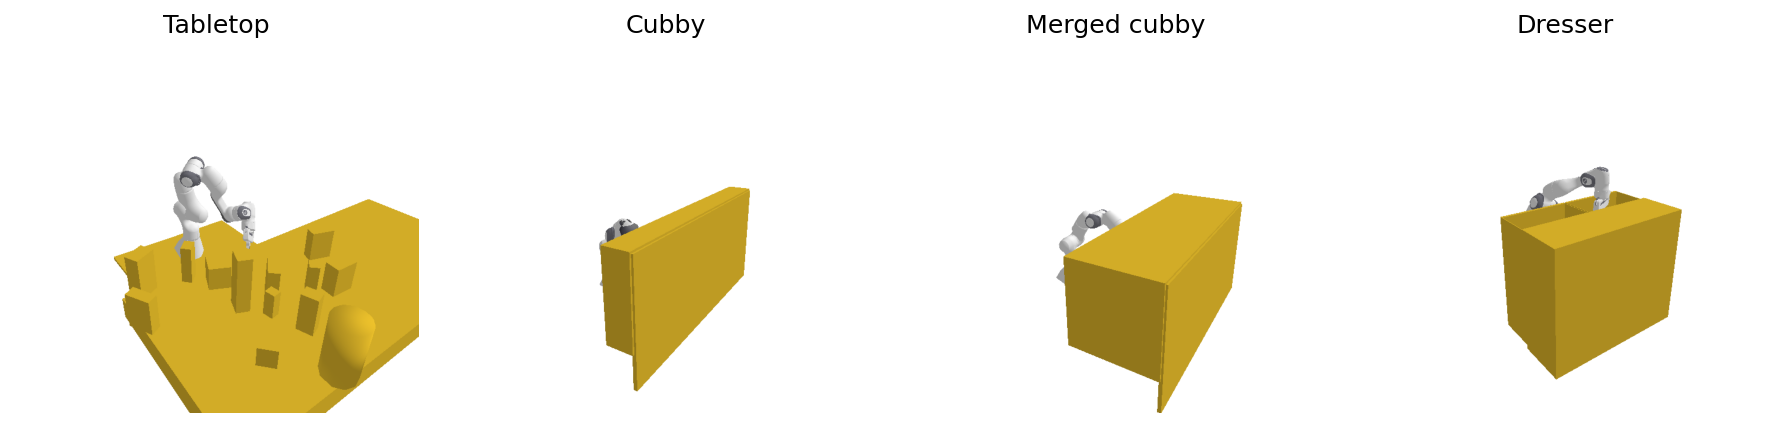
\includegraphics[width=\textwidth]{figs/env_montage.png}
\caption{The four MPiNets \cite{mpinets2022} environment types, with the Franka
Panda at a goal configuration reaching into each scene (obstacles in yellow).
Tabletop scenes scatter small objects; cubby and merged-cubby require reaching
through shelf openings; dresser requires reaching into a box---the constrained
types where swept infeasibility dominates.}
\label{fig:envs}
\end{figure*}

\section{Background and Setup}
\label{sec:setup}
\textbf{GPD.} A TemporalUNet $\epsilon$-predictor ($\sim$3.95M params) over eight
Bernstein control points, $T{=}64$, variance schedule
$\beta=\mathrm{linspace}(0,0.02,T{+}1)$; start/goal are pinned at the boundary
control points. Inference samples $K$ candidates under cost-gradient guidance
(differentiable AABB intersection-volume plus swept-volume via PyTorch forward
kinematics), then selects and stitches them \cite{gpd2025,ddpm2020}.

\noindent\textbf{Success metric.} We execute the trajectory in PyBullet under
position control; success requires \emph{no obstacle contact during execution}.
This is a continuous-execution test, not a waypoint check.

\noindent\textbf{Setup.} Unless noted, numbers are on the MPiNets
\cite{mpinets2022} \emph{hybrid}-solvable set (Fig.~\ref{fig:envs}), balanced 100
scenes per environment type (400 total), under the GPD-stitched configuration (single guide, $K{=}32$,
faithful-collision RRT-Connect stitching \cite{rrtconnect2000}). Our
re-implementation reproduces the method ordering of \cite{gpd2025} but sits
$\sim$21\pp{} below its absolute numbers; all claims below are therefore
\emph{deltas measured within our own system}, never cross-method absolutes. The
gap is not under-training (App.~\ref{app:repro}): the GPD paper releases no code or
weights and leaves $K$, guidance scale, and cost formulas unspecified, and
in-system tuning recovers only $\sim$3 of the $\sim$20\pp.

\section{The Prior Is Not the Bottleneck}
We test the five most natural prior-side improvements. Each is a clean
single-variable change sharing an identical guidance/stitching pipeline.

\subsection{Noise-schedule recalibration}
At $T{=}64$ the linear schedule gives $\bar\alpha_T\!\approx\!0.52$---the model is
never trained near pure noise, while inference starts from $\mathcal N(0,I)$. The
``fix'' (raise terminal noise, or use cosine) \emph{lowered} SR on all scene types
despite a \emph{lower} training loss ($0.53\!\to\!0.43$). The low-terminal-noise
regime keeps the reverse process near-identity, acting as an implicit smoothness
prior; injecting variance yields less-smooth, more-colliding paths.
$\epsilon$-loss is a poor proxy for planning SR.

\subsection{Polynomial capacity}
\label{sec:capacity}
Bernstein reconstruction error shows degree-7 ($n{=}8$) discards $5$--$17^\circ$ of
joint motion on the constrained demonstrations (mean $5.47^\circ$), so the
representation \emph{is} lossy where GPD struggles. Yet training $n{=}16$
($4\times$ lower reconstruction error, matched convergence loss) yields a
\textbf{net $-6.3\pp$}: it beats $n{=}8$ on sharp-turn dresser scenes but loses on
tabletop/cubby, and costs $5\times$ the training.

\noindent\textbf{Mechanism (compression $=$ smoothness regularizer).} Measuring the
raw sampled trajectories (100 scenes, before any repair), the compact $n{=}8$
prior is markedly smoother: joint-jerk RMS $0.00166$ vs.\ $0.00214$ ($-22\%$;
Fig.~\ref{fig:jerk}), with a larger clearance margin. The low-degree basis cannot
express the high-frequency motion a higher-capacity model fits, so it acts as an
implicit smoothness prior---and smoother trajectories collide less under
continuous execution. Reconstruction fidelity is \emph{anti-correlated} with the
smoothness that drives SR. Adding an explicit smoothness penalty during $n{=}16$
training (the fifth prior-side lever) recovers only $+3.4\pp$ (peak $59.2\%$ at
$\lambda{=}0.03$)---still below the $n{=}8$ baseline---confirming that the compact
basis's \emph{implicit} regularization is what the higher-capacity model lacks.

\begin{proposition}[Compactness bounds trajectory roughness]
\label{prop:compact}
For a degree-$d$ B\'ezier joint path $q(t)=\sum_{k=0}^{d} b_k B_{k,d}(t)$ with control
points $b_k$, the $m$-th derivative satisfies
$\lVert q^{(m)}\rVert_\infty \le \tfrac{d!}{(d-m)!}\,\max_k \lVert \Delta^m b_k\rVert$,
where $\Delta^m$ is the $m$-th forward difference. Hence for fixed control-point range,
a lower degree $d$ imposes a strictly smaller upper bound on velocity/acceleration/jerk:
the representation \emph{cannot} express high-frequency motion.
\end{proposition}
\noindent The bound is standard for B\'ezier hodographs; it makes the mechanism precise
--- $n{=}8$ ($d{=}7$) caps jerk more tightly than $n{=}16$ ($d{=}15$), matching the
measured $-22\%$ jerk RMS and the SR gap.

\begin{figure}[t]
\centering
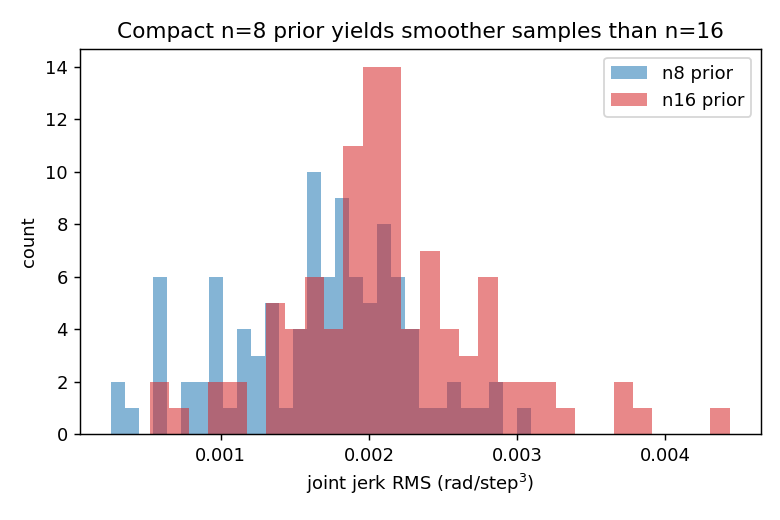
\includegraphics[width=\linewidth]{figs/smoothness_jerk.png}
\caption{Distribution of raw-sample joint jerk over 100 hybrid scenes. The compact
$n{=}8$ prior is smoother than the higher-capacity $n{=}16$ prior, a direct
mechanism for why capacity hurts SR despite lower reconstruction error.}
\label{fig:jerk}
\end{figure}

\subsection{Scene-conditioned denoiser (CFG)}
We add a masked-DeepSets \cite{deepsets2017} obstacle encoder whose embedding
feeds the time embedding, with a learned null embedding for classifier-free
guidance \cite{cfg2022}. The conditioned model reaches a \emph{lower} loss
($0.502{<}0.52$), yet with guidance removed the conditioned prior plans no better
than the scene-blind prior: scene information enters through \emph{guidance}, not
the prior. Over five paired seeds the conditioning delta is
$\mathbf{-1.75\pp}$ (95\% CI $[-2.37,-1.13]$)---a small but significant
\emph{decrease}.

\subsection{Training to convergence ($5\times$, 1M steps)}
\label{sec:train}
The most basic prior-side lever is more training. We train the canonical $n{=}8$
prior for $1{,}000{,}000$ steps ($5\times$ the baseline); $\epsilon$-loss drops
$\sim$4\% and flattens for the final 300k steps. Over five paired seeds the delta
is $\mathbf{-0.10\pp}$ (95\% CI $[-1.71,+1.51]$)---statistically zero. This rules
out under-training as the explanation for both the flat prior-side results and the
reproduction gap.

\subsection{Summary}
Five prior improvements, five nominal-metric gains, \textbf{no positive SR gain}:
deltas span statistically zero ($5\times$ training) to small significant decreases
(conditioning $-1.75\pp$; schedule and capacity larger). Against a measured
baseline sampling noise $\sigma\!\approx\!1.6\pp$, no prior intervention clears it
upward, while the repair lever below clears it by $\sim6\sigma$.

\section{Where Success Actually Comes From}
\subsection{Failure-mode analysis, and its closure}
We categorize 200 hybrid failures of the baseline, and re-categorize after repair:

\begin{center}\small
\begin{tabular}{lrr}
\toprule
failure mode & baseline \% & after repair \% \\
\midrule
success & 74.0 & 78.5 \\
goal/start IK infeasible & 2.5 & 1.5 \\
path\_collision (waypoints) & 8.0 & 17.0 \\
\textbf{dynamic\_only (swept)} & \textbf{15.5} & \textbf{3.0} \\
\bottomrule
\end{tabular}
\end{center}

\begin{figure}[t]
\centering
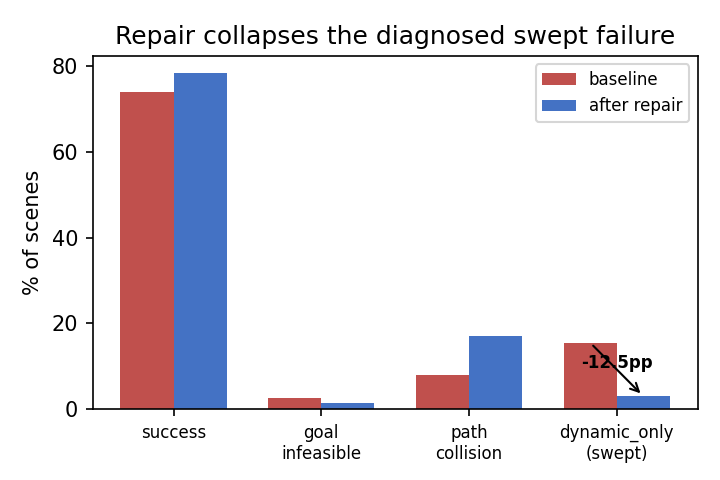
\includegraphics[width=0.92\linewidth]{figs/failure_shift.png}
\caption{Failure-mode distribution before and after repair. The dominant
baseline failure---\texttt{dynamic\_only} swept collision---collapses from
$15.5\%$ to $3.0\%$, the very failure the repair objective (Eq.~\ref{eq:repair})
targets.}
\label{fig:failshift}
\end{figure}

The executor and static checker share a contact model, so \texttt{dynamic\_only}
is genuine: the robot \emph{sweeps through obstacles between waypoints}
(Fig.~\ref{fig:failshift}). It is the
dominant residual failure, and the repair we build (\S\ref{sec:repair}) collapses
it to $3.0\%$. Of the eliminated swept failures, $\sim$4.5\pp{} convert to success
and the rest become statically-detectable \texttt{path\_collision}: on the hardest
scenes the optimizer churns but leaves a residual static collision---it converts
dynamic failures, it does not manufacture them.

\subsection{Lever 1: faithful-collision stitching}
The stitcher originally certified bridges with the loose AABB intersection-volume
\emph{proxy}, marking colliding bridges as free. Replacing it with a faithful
PyBullet check inside RRT-Connect yields \textbf{$+17.4\pp$} over the proxy plateau
($55.5{\pm}1.0\!\to\!72.9{\pm}1.6$; paired CI $[15.2,19.6]$, 5 seeds), the first
intervention to move SR.

\subsection{Lever 2: trajectory-optimization repair}
\label{sec:repair}
Motivated by the analysis above and recent work \cite{presto2025,mpd2023}, we add a
post-hoc optimizer. With endpoints $q_0,q_N$ pinned to start/goal, we solve over
the interior waypoints $q_{1:N-1}$
\begin{equation}
\begin{aligned}
\min_{q_{1:N-1}}\ &\textstyle\sum_{i} c(q_i)
  + \lambda_m \sum_i c\big(\tfrac{q_i+q_{i+1}}{2}\big)\\[-1pt]
  &\textstyle + \lambda_s \sum_i \lVert q_{i-1}-2q_i+q_{i+1}\rVert^2,
\end{aligned}
\label{eq:repair}
\end{equation}
where $c(\cdot)$ is the guide's differentiable collision cost. The first term
drives waypoints out of collision; the second penalizes collision at
\emph{edge-midpoints}, directly targeting the swept infeasibility diagnosed above;
the third is a smoothness (acceleration) penalty. We run Adam with joint-limit
projection and \emph{early-stop} on a densified faithful collision check, returning
a densified trajectory for overshoot-free execution. It reuses the existing
differentiable cost---no retraining.

Over five seeds, repair raises SR from $72.9{\pm}1.6$ to $81.8{\pm}1.3$: a paired
\textbf{$+8.9\pp$, 95\% CI $[7.6,10.2]$}, $t(4){=}19.4$, $p{<}0.0001$. The
optimizer targets a densified static check; the benchmark independently verifies
dynamic execution, so this is a real executable-SR gain at $\sim$$+1.8$s/scene
(only on scenes needing repair).

\begin{table}[t]\centering\small
\caption{Main results: the two feasibility levers stack, on two planners (hybrid 400,
continuous-execution SR). Every $\Delta$ is paired with a 95\% CI ($^{\dagger}$5 seeds,
$^{\ddagger}$3 seeds); the prior-side interventions (\S\ref{sec:capacity}--\ref{sec:train})
by contrast never clear the $\sigma{\approx}1.6\pp$ noise floor.}
\label{tab:main}
\begin{tabular}{llcc}
\toprule
planner & pipeline & SR\% & $\Delta$ (CI) \\
\midrule
\multirow{3}{*}{GPD}
 & AABB-proxy stitch      & $55.5{\pm}1.0$ & --- \\
 & \;$+$ faithful stitch$^{\dagger}$  & $72.9{\pm}1.6$ & $+17.4$ $[15.2,19.6]$ \\
 & \;$+$ trajopt repair$^{\dagger}$   & $\mathbf{81.8{\pm}1.3}$ & $+8.9$ $[7.6,10.2]$ \\
\midrule
\multirow{2}{*}{EDMP}
 & base                   & $57.2{\pm}1.0$ & --- \\
 & \;$+$ trajopt repair$^{\ddagger}$  & $\mathbf{64.8{\pm}1.3}$ & $+7.6$ $[5.2,9.9]$ \\
\bottomrule
\end{tabular}
\end{table}

\subsection{Is the prior even needed? A naive-seed control}
\label{sec:naive}
If improving the prior never helps, is the prior irrelevant? We replace the
diffusion candidates with a single straight-line joint-space seed and run the
\emph{identical} downstream (RRT stitch $\pm$ repair):

\begin{center}\small
\begin{tabular}{lrr}
\toprule
seed & stitch only & stitch $+$ repair \\
\midrule
linear (no prior) & $18.5{\pm}0.3$ & $55.0{\pm}1.0$ \\
diffusion (prior) & $72.9{\pm}1.6$ & $81.8{\pm}1.3$ \\
\bottomrule
\end{tabular}
\end{center}

The prior is \textbf{necessary as an initializer}: even the best repair on a linear
seed reaches only $55\%$, $-26.8\pp$ below diffusion$+$repair---repair cannot
substitute for a competent seed. Yet repair does far more \emph{work} on the bad
seed ($+36.5\pp$) than on the diffusion seed ($+8.9\pp$): good initialization and
good repair are complementary, not interchangeable. This scopes the paper's claim
precisely---\emph{improving} an already-competent prior buys nothing, but the prior
is not dispensable.

\subsection{The repair lever generalizes (EDMP)}
\label{sec:edmp}
If the bottleneck is the feasibility machinery, the same repair should help a
different planner. Applied unchanged to EDMP \cite{edmp2024} (a different model:
$T{=}255$ over full 50-waypoint trajectories), repair lifts SR from
$57.2{\pm}1.0$ to $64.8{\pm}1.3$ ($\mathbf{+7.6\pp}$, paired CI $[5.2,9.9]$,
3 seeds)---a significant gain on the same constrained scene types, at
$\sim$$+7$s/scene. The lever is planner-agnostic.

\subsection{Generalization across datasets}
\begin{figure}[t]
\centering
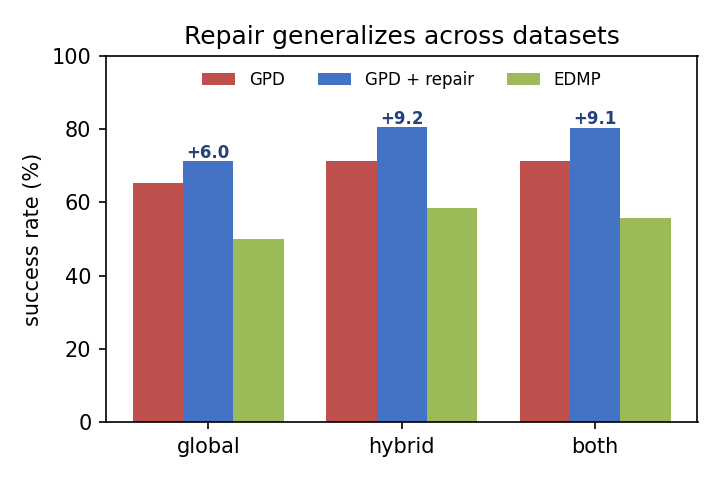
\includegraphics[width=0.92\linewidth]{figs/cross_dataset.png}
\caption{Repair generalizes across all three MPiNets solvable splits ($+6$ to
$+9\pp$), and GPD$+$repair beats EDMP everywhere at a fraction of its planning
time (Table below).}
\label{fig:crossds}
\end{figure}
The repair lever is not a hybrid-only artifact (Fig.~\ref{fig:crossds}). On the
three MPiNets solvable splits (600 natural-weighted scenes each), it lifts SR by
$+6$ to $+9\pp$ everywhere, and consistently beats EDMP at a fraction of its
planning time:

\begin{center}\small
\begin{tabular}{lccc}
\toprule
split & GPD & GPD$+$repair & EDMP \\
\midrule
global & 65.2 & \textbf{71.2} \,($+6.0$) & 50.0 \\
hybrid & 71.3 & \textbf{80.5} \,($+9.2$) & 58.5 \\
both   & 71.2 & \textbf{80.3} \,($+9.1$) & 55.7 \\
\midrule
avg time & 7.6s & 9.4s & 47.6s \\
\bottomrule
\end{tabular}
\end{center}

\noindent The gain is largest on the constrained (hybrid/both) splits where swept
infeasibility dominates, consistent with the failure-mode diagnosis.

\section{Discussion}
The two effective levers are both on the \emph{inference-time feasibility
machinery}, and both concern \emph{continuous} feasibility (collision-free bridges;
collision-free swept motion). The ineffective levers are all on the prior, and
several improved nominal generative metrics. A recurring theme is that
\emph{fidelity is decoupled from success at every level}: $\epsilon$-loss (priors),
reconstruction error (capacity), and even the differentiable repair \emph{objective}
(an exact sphere-SDF objective ties the cheap AABB proxy; App.~\ref{app:sphere}),
because the faithful check is the true oracle. For guided diffusion planners,
effort spent improving priors yields little once a competent guided prior exists;
the returns are in feasibility repair.

\noindent\textbf{When would the prior matter?} Our claim is scoped, not absolute.
The naive-seed control (\S\ref{sec:naive}) shows the prior is indispensable as an
initializer---remove it and repair stalls at 55\%---so a prior good enough to place
the seed in roughly the right homotopy class is a prerequisite, not a target for
further tuning. We expect prior improvements to pay off in regimes our benchmark
does not stress: much higher-DoF systems, tasks with hard end-effector constraints
the guidance cost cannot express, or settings without a fast faithful collision
checker to serve as the repair oracle. Absent those, the empirical picture is
stark---five prior-side changes, no gain; two feasibility changes, double-digit
gains.

\noindent\textbf{On reporting negative results.} Every intervention here is measured
under one continuous-execution metric with multi-seed confidence intervals and paired
tests---rigor that lets a null (\S\ref{sec:train}: $5\times$ training, $\Delta{=}{-}0.1\pp$)
be read as a finding rather than noise, following recent calls for empirical rigor and
the reporting of negative results \cite{emprobot2024,negresults2024}.

\noindent\textbf{Limitations.} Core results are on hybrid-solvable, balanced 400;
we generalize the repair lever to global/both splits and to EDMP, but larger $N$,
a second robot embodiment, and a real-robot study would tighten the claim (future work).
Absolute SR is below the published GPD system; we therefore report deltas within a fixed
system rather than cross-method absolutes.

\section{Conclusion}
In a controlled study of guided polynomial diffusion planning, the generative
prior is not the bottleneck: five natural prior improvements never raise SR while
improving nominal metrics, and a $5\times$ prior changes nothing. The gains live in
the feasibility machinery---faithful-collision stitching ($+17.4\pp$) and
trajectory-optimization repair ($+8.9\pp$ on GPD, $+7.6\pp$ on EDMP)---which also
collapses the diagnosed swept-collision failure. The prior earns its place as a
necessary initializer, not as a tunable lever. We release the implementation and
all ablations to support feasibility-centric research on diffusion planners.

\appendix
\section{Ablations}
\subsection{Trajopt hyperparameters (time/accuracy Pareto)}
\label{app:hyper}
\begin{figure}[t]
\centering
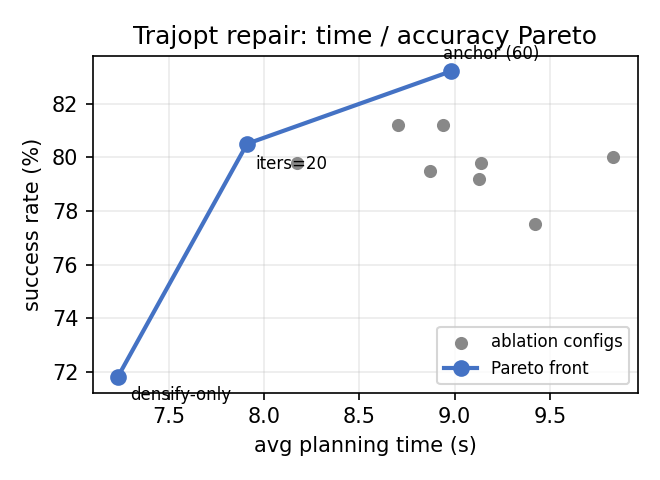
\includegraphics[width=0.86\linewidth]{figs/pareto.png}
\caption{Time/accuracy trade-off of the trajopt-repair configurations. The Pareto
front runs densify-only $\to$ iters~20 $\to$ the anchor (iters~60); all other
settings are dominated.}
\label{fig:pareto}
\end{figure}
One-factor-at-a-time around the default (iters 60, densify 3, midpoint-weight 1.0),
hybrid 400 (Fig.~\ref{fig:pareto}). \emph{Iterations peak, not plateau}: SR
saturates by $\sim$40 and iters 100 regresses ($-3.2\pp$)---over-optimization
drifts waypoints off the smooth seed. The \emph{midpoint} term is causal for swept
feasibility ($-3.4\pp$ without it). Output densification peaks at 3.

\begin{center}\small
\begin{tabular}{llrr}
\toprule
knob & value & SR\% & avg t (s) \\
\midrule
iters & 0 (densify-only) & 71.8 & 7.2 \\
      & 20 & 80.5 & 7.9 \\
      & 40 & 81.2 & 8.7 \\
      & \textbf{60} & \textbf{83.2} & 9.0 \\
      & 100 & 80.0 & 9.8 \\
\midrule
out-densify & 1 & 77.5 & 9.4 \\
            & \textbf{3} & \textbf{83.2} & 9.0 \\
            & 5 & 79.5 & 8.9 \\
\midrule
mid-weight & 0.0 & 79.8 & 8.2 \\
           & \textbf{1.0} & \textbf{83.2} & 9.0 \\
           & 2.0 & 81.2 & 8.9 \\
\bottomrule
\end{tabular}
\end{center}

\subsection{Exact vs.\ proxy collision objective}
\label{app:sphere}
We implemented an exact GPU-batched sphere-SDF objective (FK-placed link spheres
vs.\ oriented obstacle boxes), removing the AABB double-inflation. Swapped into the
same repair loop (3 seeds) it gives $82.0{\pm}0.9$ vs.\ $81.8{\pm}1.3$ for the
proxy---a paired $+0.6\pp$, not significant, at equal time. Because the faithful
PyBullet check is the stopping oracle, objective fidelity is not a lever.

\subsection{Per-intervention seed CIs}
\label{app:seeds}
Five paired seeds, hybrid 400. Baseline $72.9{\pm}1.6$; conditioning
$71.2{\pm}1.3$ ($\Delta{=}{-}1.75$, CI $[-2.37,-1.13]$); $5\times$ training
$72.8{\pm}0.9$ ($\Delta{=}{-}0.10$, CI $[-1.71,+1.51]$); repair $81.8{\pm}1.3$
($\Delta{=}{+}8.9$, CI $[7.6,10.2]$).

\subsection{Reproduction study: how far in-system tuning closes the gap}
\label{app:repro}
Our re-implementation reproduces the GPD paper's method ordering but sits
$\sim$21\pp{} below its absolute numbers (\S\ref{sec:setup}). Because all our
contributions are within-system deltas, absolute matching is not required; this
study asks how much of the gap is recoverable in-system and attributes the residual.
Crucially, the GPD paper releases \textbf{no code and no weights}, and leaves the
guidance scale, candidate count $K$, and collision-cost formulas unspecified---so an
exact match is not reconstructable from the paper. Training is not the cause: our
budget already matches theirs (20k steps, same 6.54M Bernstein set), and
$5\times$/1M-step training moves SR by $-0.1\pp$ (\S\ref{app:seeds}).

Sweeping the two documented levers on the GPD-stitched config (hybrid, 400 scenes;
Fig.~\ref{fig:repro}):

\begin{center}\small
\begin{tabular}{lrr}
\toprule
config & SR\% & avg t (s) \\
\midrule
baseline (K=32, scale 1) & 73.2 & 7.3 \\
K=64 & 69.8 & 8.4 \\
K=128 & \textbf{76.5} & 10.9 \\
K=32, scale 2 & 76.0 & 7.3 \\
K=32, scale 3 & 72.8 & 7.3 \\
K=128, scale 3 & \textbf{76.5} & 10.9 \\
K=32 + sphere-SDF guidance & 67.2 & 3.4 \\
K=128 + sphere-SDF guidance & 72.0 & 4.1 \\
\midrule
\emph{GPD paper (unreleased weights/config)} & \emph{92.8} & \emph{1.9} \\
\bottomrule
\end{tabular}
\end{center}

Raising the candidate budget to $K{=}128$ and the guidance scale to $2\times$ each
add $\sim$$3\pp$, plateauing at $\mathbf{76.5\%}$ --- recovering only $\sim$3 of the
$\sim$20\pp{} gap. Replacing the guide's inflated-AABB gradient with our exact
sphere-SDF gradient (App.~\ref{app:sphere}) as the \emph{denoising guidance} is
\emph{worse} ($-6\pp$): the guide's clearance/expansion schedule supplies a safety
margin that geometric exactness does not, a further instance of objective-fidelity
being decoupled from SR. The residual $\sim$16\pp{} is thus attributable to factors
we cannot reconstruct from the paper --- the tuned 7-cost guidance ensemble (whose
$1G\!\to\!7G$ gain we reproduce at $+6\pp$ vs.\ the paper's $+18\pp$), the exact
guidance scale, and the authors' trained weights. This confirms that absolute
cross-method comparison is unavailable here and that our within-system deltas are the
sound unit of claim.

\begin{figure}[t]
\centering
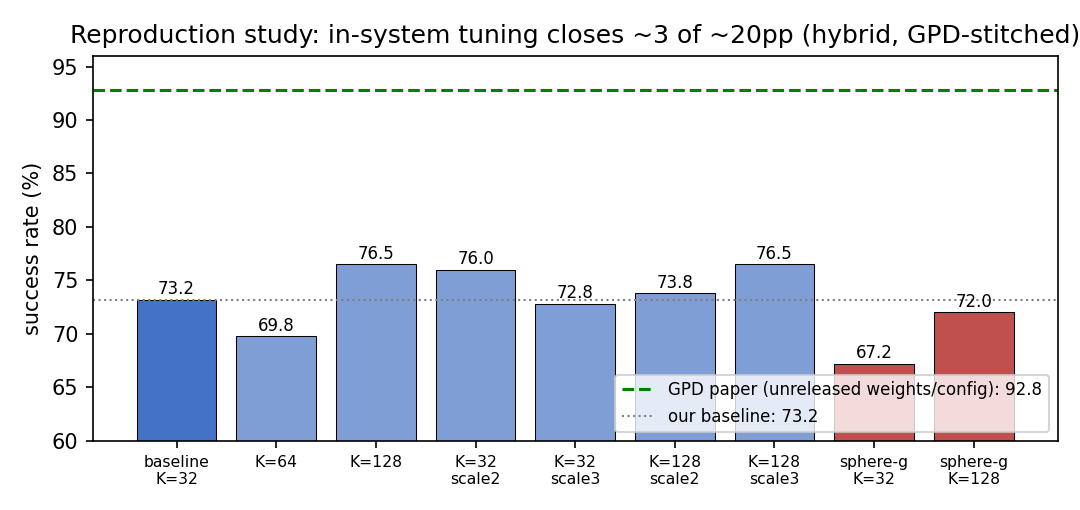
\includegraphics[width=\linewidth]{figs/reproduction_curve.png}
\caption{Reproduction study on the GPD-stitched config (hybrid). In-system candidate
and guidance-scale tuning recovers only $\sim$3 of the $\sim$20\pp{} gap to the GPD
paper (green, unreleased weights/config); exact sphere-SDF guidance (red) is worse.}
\label{fig:repro}
\end{figure}

\subsection{Continuous-feasibility audit and a dense repair objective}
\label{app:continuous}
The dominant failure (\S\ref{sec:setup}, App.~\ref{app:seeds}) is \emph{swept}
infeasibility, yet the executor and our checks only sample the path discretely.
Differentiable swept-volume models exist \cite{svsdf2024,neuralsvcd2025} but none are
used inside a diffusion planner's repair loop; likewise safe-diffusion methods
\cite{safediffuser2025} enforce constraints only at sampled points. We therefore (i)
\emph{audit} continuous feasibility at increasing check resolution $R$ (samples per
edge), and (ii) test a \emph{dense} repair objective that evaluates collision at $S$
interpolated sub-configs per edge (the \S\ref{sec:repair} midpoint is $S{=}1$).

\begin{figure}[t]
\centering
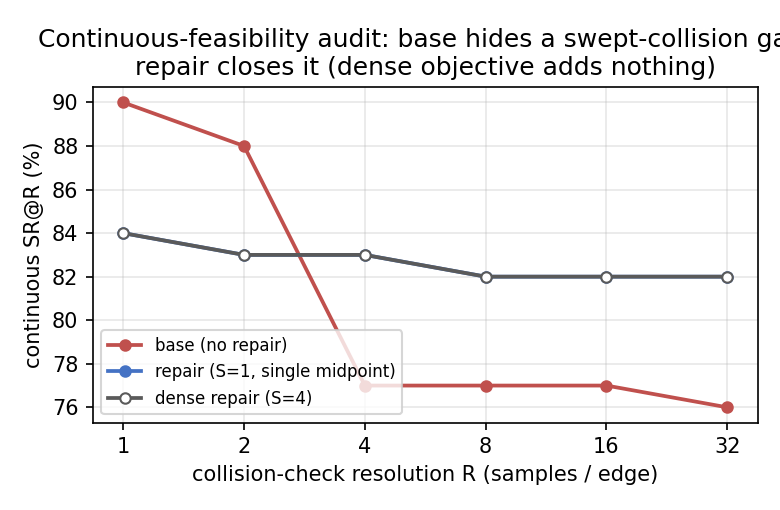
\includegraphics[width=0.92\linewidth]{figs/continuous_audit.png}
\caption{Continuous-feasibility audit (100 hybrid scenes). The base planner's
success rate collapses as the collision check densifies ($90\%$ at waypoints
$\to76\%$ at $R{=}32$): $\sim$14\pp{} of ``waypoint-free'' plans actually sweep
through obstacles. Repair nearly eliminates this ($84\!\to\!82\%$, flat), and a
dense $S{=}4$ objective coincides exactly with the single-midpoint $S{=}1$ repair.}
\label{fig:continuous}
\end{figure}

\noindent\textbf{The audit exposes a real swept gap, which repair closes.}
Fig.~\ref{fig:continuous}: the \emph{base} planner is $90\%$ feasible at waypoints
but only $76\%$ under a dense ($R{=}32$) continuous check --- roughly a seventh of
nominally-free plans sweep through obstacles between waypoints. Trajectory-repair is
nearly \emph{resolution-flat} ($84\!\to\!82\%$): it produces genuinely
continuous-feasible paths, not just waypoint-free ones.

\noindent\textbf{But a denser repair objective does not help.} Over 5 seeds
(hybrid 400): $S{=}1$ gives $81.8{\pm}1.3$, $S{=}4$ gives $81.7{\pm}1.3$ --- a paired
$-0.15\pp$ (95\% CI $[-0.79,+0.49]$) --- while costing $+2.5$s/scene ($9.0\!\to\!11.4$s;
$S{=}8$ is $14.8$s). The single-midpoint swept term is already a sufficient statistic
for continuous feasibility: because repair early-stops on a \emph{densified faithful}
oracle, a denser \emph{differentiable} objective changes nothing --- the same
objective-fidelity$\perp$SR decoupling seen for the noise schedule, capacity, and the
exact sphere-SDF objective (App.~\ref{app:sphere}). Continuous feasibility is worth
\emph{measuring} and \emph{repairing}, but not worth a heavier objective.

\noindent\textbf{The audit generalizes across datasets, and is representation-dependent
across planners.} Fig.~\ref{fig:auditcross} (mean$\pm$std over seeds): base GPD's
waypoint$\to$dense gap is large and significant on all three splits ---
$25.0{\pm}1.7$ / $17.4{\pm}2.6$ / $20.3{\pm}1.2\pp$ on global/hybrid/both. For EDMP,
whose longer diffusion chain acts on full 50-waypoint trajectories (denser inter-waypoint
motion), the gap is small and not significant ($4.2{\pm}5.2\pp$) --- so the
over-reporting is most acute for compact bases like GPD's degree-7 B\'ezier. In every
case repair flattens the curve and dynamic execution tracks the dense static check. This
makes the audit a general evaluation-rigor prescription: learned planners should report
success at a stated continuous-check resolution (classical planners already do
\cite{rrtconnect2000}), not at the waypoints alone.

\begin{figure*}[t]
\centering
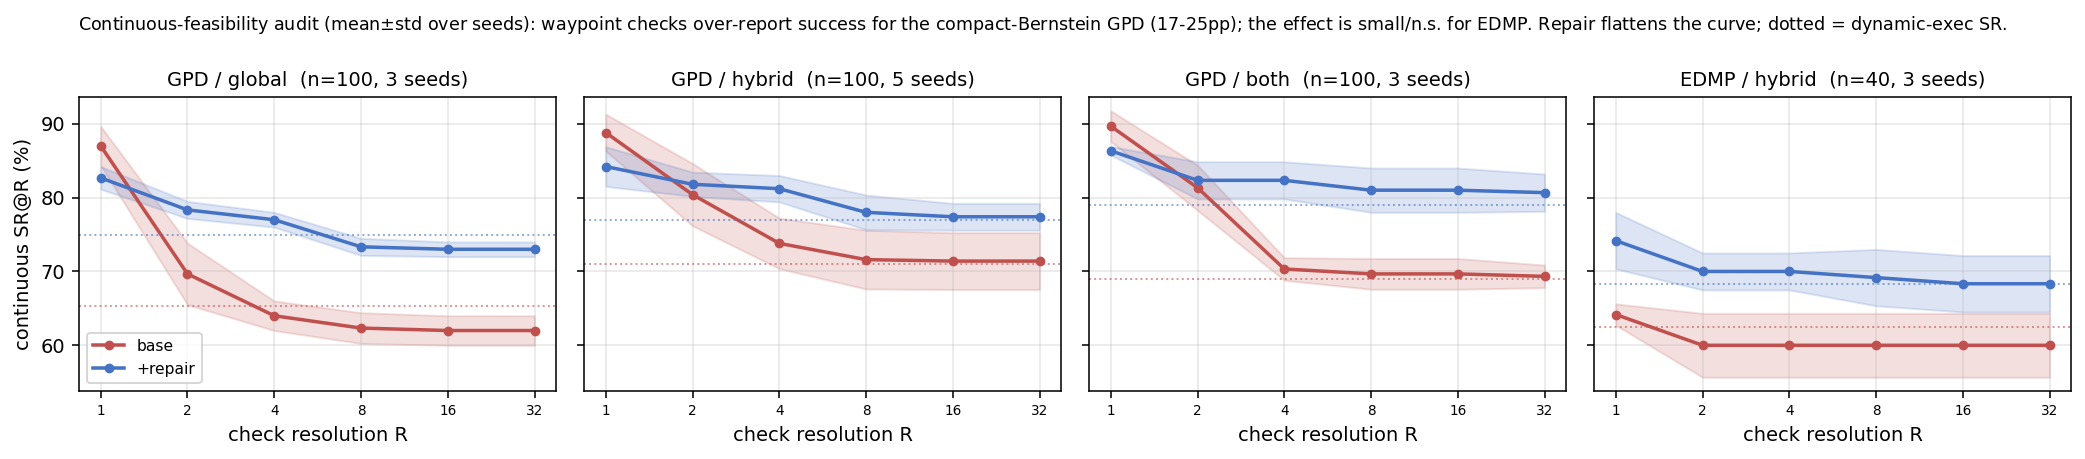
\includegraphics[width=0.98\textwidth]{figs/continuous_audit_cross.png}
\caption{Continuous-feasibility audit across datasets (GPD: global/hybrid/both) and a
second planner (EDMP). Base (red) success collapses as the check densifies; repair
(blue) is nearly resolution-flat; dotted lines are dynamic-execution SR ($\approx$ the
dense static check). The waypoint$\to$dense over-reporting is $10$--$27\pp$.}
\label{fig:auditcross}
\end{figure*}

\subsection{Can the feasibility lever be shortcut? A survey of negative levers}
\label{app:levers}
We tested six literature-motivated ways to improve or replace the stitch$+$trajopt
machinery. None significantly exceeds plain oracle-gated repair
(Table~\ref{tab:levers}); the three we have not yet detailed are below.

\begin{table}[t]\centering\small
\caption{Every attempt to improve or shortcut the feasibility machinery, vs.\ the
oracle-gated trajopt-repair baseline ($81.8{\pm}1.3$, hybrid 400). No lever clears it
significantly. ``$\Delta$'' is paired; $^{\dagger}$5 seeds, $^{\ddagger}$3 seeds.}
\label{tab:levers}
\begin{tabular}{lccl}
\toprule
lever & SR\% & $\Delta$ vs.\ repair & verdict \\
\midrule
denser repair objective ($S{=}4$)$^{\dagger}$ & $81.7$ & $-0.15$ & tie \\
exact sphere-SDF objective$^{\ddagger}$        & $82.0$ & $+0.58$ & tie (n.s.) \\
sphere-SDF \emph{guidance}$^{\dagger}$          & $\sim$76 & $\sim{-}6$ & worse \\
verifier best-of-$K$ ($K{=}128$)$^{\dagger}$    & $83.5$ & $+1.65$ & tie (n.s.) \\
learned amortized repair$^{\dagger}$            & $64.2$ & $-17.6$ & worse \\
SMC particle steering$^{\dagger}$               & $80.8$ & $-1.0$  & tie (n.s.) \\
\bottomrule
\end{tabular}
\end{table}

\noindent\textbf{Verifier-guided selection (best-of-$K$ by the faithful oracle).} Since
the faithful PyBullet oracle---not the differentiable cost---gates success, we select
the candidate with the highest densified free-fraction (a best-of-$N$ verifier
\cite{robomonkey2025}) rather than the guide's cost. At $K{=}32$ this \emph{underperforms}
guide-cost$+$RRT-stitch ($-3.4\pp$ with repair, 5 seeds), because stitching \emph{bridges}
colliding segments across candidates while selection keeps only one. Its value scales
with $K$ (Fig.~\ref{fig:alloc}): at $K{=}128$ oracle-selection$+$trajopt reaches
$83.5{\pm}1.0$ vs.\ the $81.8{\pm}1.3$ trajopt baseline --- a paired $+1.65\pp$ (95\% CI
$[-1.0,+4.3]$, \emph{not significant}) at $+3$s/scene. A compute-optimal-allocation grid
over $K$, guidance, and repair iterations (per-component wall-clock: diffusion dominates
at $\sim$7--10s, repair $\sim$1--3s, selection $<0.5$s) shows the Pareto front prefers
oracle-selection but the frontier does not clear the trajopt baseline by a significant
margin.

\begin{figure}[t]
\centering
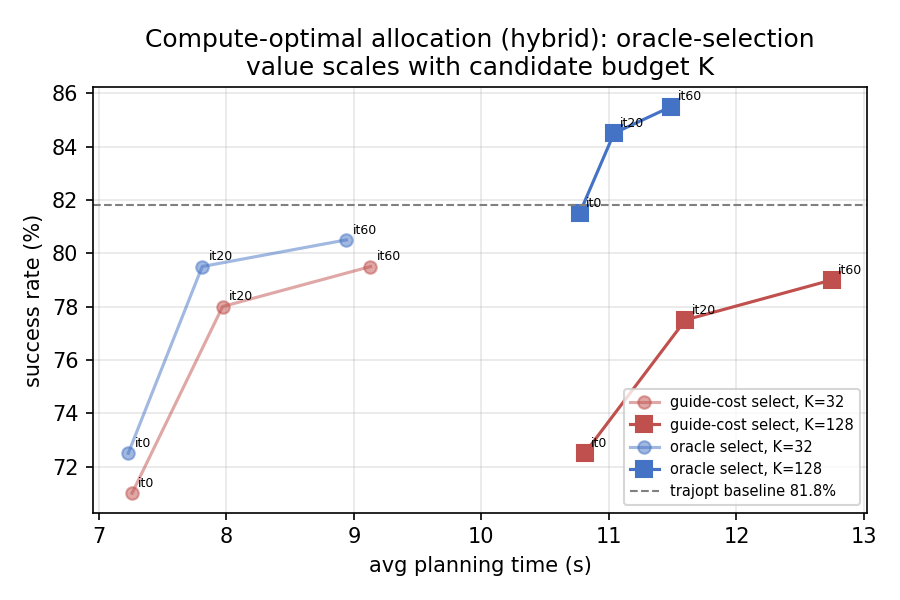
\includegraphics[width=0.9\linewidth]{figs/compute_allocation.png}
\caption{Compute-optimal allocation (hybrid). Oracle (verifier) selection's benefit
grows with candidate budget $K$, but the 5-seed confirmation of the best point
($K{=}128$, +trajopt) is $83.5{\pm}1.0$ --- statistically tied with the trajopt
baseline (dashed) at higher cost.}
\label{fig:alloc}
\end{figure}

\noindent\textbf{Learned amortized repair.} We distilled the iterative trajopt into a
one-shot network (stitched seed $+$ obstacle set $\to$ residual repair; DeepSets scene
encoder, endpoints pinned) from $1800$ (seed, repaired) pairs, to reclaim latency
\cite{presto2025}. It \emph{fails}: held-out regression loss exceeds the identity
(copy-the-seed) baseline, and in the pipeline one-shot learned repair scores
$64.2\pm2.1$ --- \emph{worse than no repair} ($-8.7\pp$) --- while a learned$+$trajopt
warm-start hybrid reaches only $75.6\pm1.8$ ($<$ the $81.8$ trajopt baseline) at barely
lower latency. Distillation from this data budget does not generalize; the iterative
oracle-gated optimization remains necessary.

\noindent\textbf{Oracle-in-the-loop SMC steering.} We also steer the reverse diffusion as a particle filter: in the chain's second half we resample the $K$ particles by a sphere-SDF feasibility potential (Feynman-Kac / twisted-SMC steering), concentrating them in feasible modes as they form. This too fails: $-3.2\pp$ on the base pipeline (5 seeds; resampling collapses the candidate diversity RRT-stitch needs) and a non-significant $-1.0\pp$ with trajopt. 

\noindent\textbf{Synthesis.} Across six attempts to improve or shortcut the feasibility
machinery (Table~\ref{tab:levers}) --- denser continuous objective, exact sphere-SDF
objective, sphere-SDF guidance, verifier-guided selection, learned amortized repair, and
SMC particle steering --- none significantly exceeds plain oracle-gated trajopt repair. The lever is robust; the returns are in \emph{using}
the faithful oracle inside stitch/repair, not in a heavier objective, a cleverer
selector, or a distilled shortcut.

\subsection{Positioning vs.\ published systems}
\label{app:positioning}
Table~\ref{tab:position} places our within-system results next to published numbers.
We never compare across the two blocks as a claim: our absolute SR sits $\sim$21\pp{}
below the published GPD system (App.~\ref{app:repro} attributes this to the unreleased
7-cost guidance ensemble and trained weights, not to under-training or our repair). The
table's purpose is orientation---GPD$+$repair is fast and repair-dominated, EDMP is an
order of magnitude slower, and classical cuRobo occupies a different speed/quality point.

\begin{table}[t]\centering\small
\caption{Positioning. \emph{Top}: our re-implementation (within-system, comparable).
\emph{Bottom}: published numbers under each paper's own protocol (\emph{reference only};
not directly comparable---different collision checks, scene draws, and unreleased
weights).}
\label{tab:position}
\begin{tabular}{llcc}
\toprule
& system & SR\% & time \\
\midrule
\multirow{3}{*}{ours}
 & GPD (stitched)      & $72.9{\pm}1.6$ & $7.6$s \\
 & GPD $+$ repair      & $81.8{\pm}1.3$ & $9.4$s \\
 & EDMP $+$ repair     & $64.8{\pm}1.3$ & $\sim$51s \\
\midrule
\multirow{3}{*}{\shortstack[l]{published\\(ref.)}}
 & GPD \cite{gpd2025}       & $92.8$ & $1.9$s \\
 & M$\pi$Nets \cite{mpinets2022} & $75.8$ & --- \\
 & cuRobo \cite{curobo2023} & $\sim$99 & $\sim$0.1s \\
\bottomrule
\end{tabular}
\end{table}

\subsection{Released benchmark and audit protocol}
\label{app:release}
To make the study reusable, we release: (i) the GPU-native GPD/EDMP re-implementation
with all ablation configs; (ii) the balanced 400-scene hybrid evaluation set (and the
global/both splits) with the continuous-execution success metric; and (iii) the
\emph{continuous-feasibility audit protocol}---the SR@$R$ harness (\S\ref{app:continuous})
that measures how much reported success survives a dense collision check, plus the
oracle-gated repair module. The audit is a drop-in evaluation any learned planner can
run; we recommend reporting SR at a stated check resolution rather than at waypoints
alone, matching classical practice \cite{rrtconnect2000}.

\small
\bibliographystyle{plain}
\bibliography{refs}

\end{document}
